\chapter{Lecture 10: Magnetic Fields, Gauge Invariance, and Circular Motion}

These notes follow Leonard Susskind's tenth lecture on particles in magnetic fields, preserving the order in which the ideas are introduced and tested. The lecture begins with a recap of magnetic fields as position-dependent vector fields, narrows immediately to static fields, and then builds an action principle for a charged particle in a magnetic background. Preserved lecture frames, curated through LazyingArt LLC and Video2Book, are kept where the board layout or a live derivation matters; the transcript remains the primary source of truth. Electric fields are mentioned at the start, but the lecture quickly sets them aside and concentrates on the magnetic problem.

\section{Magnetic Fields, Constraints, and the Static Setup}

We begin exactly where the lecture begins: there are electric and magnetic fields, and they are vector fields. A magnetic field depends on position, has direction and magnitude, and may be written either as \(\mathbf B(\mathbf x)\) or in component form as \(B_i(\mathbf x)\), namely \(B_x\), \(B_y\), and \(B_z\). The first frame from the board is useful here, not because every chalk mark is perfectly legible, but because it records the sequence of ideas: component language first, constraint second, and the vector potential third.

\begin{figure}[htbp]
\centering

\includegraphics[width=0.78\textwidth]{lecture_10_figure_02.png}
\caption{Divergence-free magnetic field and vector potential.}
\end{figure}

For the purposes of this lecture we make a definite simplifying assumption: the electric and magnetic fields, if present, are static. They have no explicit time dependence. This is not a fundamental restriction, only a choice that keeps the mechanics transparent.

The first real physical fact is the no-monopole constraint. In ordinary classical electrodynamics there are no magnetic sources, and therefore
\begin{align}
\nabla\!\cdot\!\mathbf B = 0.
\end{align}
This is a restriction on the allowed magnetic fields. Not every vector field qualifies as a magnetic field; only those with vanishing divergence do.

At once the lecture asks for a way to implement this automatically. It would be inconvenient to keep checking \(\nabla\!\cdot\!\mathbf B=0\) every time we write down a magnetic field. So we introduce a new object, the vector potential \(\mathbf A\), by
\begin{align}
\mathbf B = \nabla\times \mathbf A.
\end{align}
The point is the elementary identity
\begin{align}
\nabla\!\cdot\!(\nabla\times \mathbf A)=0.
\end{align}
Once \(\mathbf B\) is written as a curl, the constraint is built in. That is the first major pivot of the lecture.

\section{Vector Potential and Gauge Freedom}

As soon as \(\mathbf A\) appears, a price is paid: \(\mathbf A\) is not unique. If \(S(\mathbf x)\) is any scalar field, then
\begin{align}
\mathbf A \longrightarrow \mathbf A+\nabla S
\end{align}
does not change the magnetic field, because
\begin{align}
\nabla\times(\nabla S)=0.
\end{align}
Thus different vector potentials can describe exactly the same magnetic field. This is gauge freedom. The lecture turns that ambiguity into a principle: the physically meaningful quantities must be gauge invariant.

It is characteristic of the lecture not to leave this in abstract form. We are immediately given a worked example, which will later be reused as a computational tool. The intended field, despite a momentary spoken self-correction, is
\begin{align}
\mathbf B=(0,0,B)=B\,\hat z.
\end{align}
A first gauge for this uniform field is
\begin{align}
A_x=0,\qquad A_y=Bx,\qquad A_z=0.
\end{align}
Checking it is easy:
\begin{align}
B_z=\frac{\partial A_y}{\partial x}-\frac{\partial A_x}{\partial y}=B.
\end{align}
A second gauge is
\begin{align}
A_x=-By,\qquad A_y=0,\qquad A_z=0,
\end{align}
and now
\begin{align}
B_z=\frac{\partial A_y}{\partial x}-\frac{\partial A_x}{\partial y}=0-(-B)=B.
\end{align}
So the two vector potentials produce the same magnetic field.

The lecture then asks for the gauge transformation that connects them. Rather than search for it, we write one down:
\begin{align}
S=Cxy.
\end{align}
Its gradient is
\begin{align}
\nabla S=(Cy,Cx,0).
\end{align}
If we begin with \(A_x=0\), \(A_y=Bx\), \(A_z=0\), then after the transformation \(\mathbf A\to\mathbf A+\nabla S\) we have
\begin{align}
A_x'&=Cy, &
A_y'&=(B+C)x, &
A_z'&=0.
\end{align}
Choosing \(C=-B\) gives
\begin{align}
A_x'=-By,\qquad A_y'=0,\qquad A_z'=0,
\end{align}
which is exactly the second gauge.

The lecture then chooses \(C=-\frac{B}{2}\), leading to the more symmetric representative
\begin{align}
A_x=-\frac{B}{2}y,\qquad A_y=\frac{B}{2}x,\qquad A_z=0.
\end{align}
This third gauge is only partly verbalized in the lecture, so it is best presented cautiously as the natural completion of the computation already underway.

What matters here is not only that the gauges are equivalent, but that different gauges reveal different structures. The lecture pauses to stress that some property may be obvious in one gauge and obscure in another. That point will later pay off when we solve the motion in a uniform field.

\section{The Magnetic Lagrangian and Gauge Invariance of the Action}

Only after gauge freedom has been made concrete do we return to mechanics. The lecture writes down the Lagrangian for a point particle moving in a fixed static magnetic field. This is not yet the action for the electromagnetic field itself; it is the action for the particle in a prescribed background:
\begin{align}
L
=
\frac{1}{2}m\left(\dot x^2+\dot y^2+\dot z^2\right)
+\frac{e}{c}\left(A_x\dot x+A_y\dot y+A_z\dot z\right).
\end{align}
Equivalently,
\begin{align}
L=\frac{1}{2}mv^2+\frac{e}{c}\,\mathbf A\cdot \mathbf v.
\end{align}

\begin{figure}[htbp]
\centering

\includegraphics[width=0.86\textwidth]{lecture_10_figure_03.png}
\caption{Lagrangian with vector-potential coupling.}
\end{figure}

The board evidence matters here because Susskind writes the interaction term out component by component. He does not treat \(\mathbf A\cdot\mathbf v\) as a black box. That is the right preparation for the algebra still to come.

Before deriving any equations of motion, the lecture revisits gauge invariance at the level of the action. Under
\begin{align}
A_i \longrightarrow A_i+\partial_i S,
\end{align}
the action changes by
\begin{align}
\delta I
=
\frac{e}{c}\int \partial_i S\,\dot x^i\,dt.
\end{align}
Now along a trajectory
\begin{align}
\frac{dS}{dt}=\partial_i S\,\dot x^i,
\end{align}
so
\begin{align}
\delta I
=
\frac{e}{c}\int \frac{dS}{dt}\,dt
=
\frac{e}{c}\big(S_f-S_i\big).
\end{align}
Thus the action is not strictly gauge invariant; it changes by an endpoint term.

\subsection{Question \& Answer}

\paragraph{Question.} If the action changes under a gauge transformation, why are the equations of motion still gauge invariant?

\paragraph{Answer.} In the variational principle the endpoints are held fixed. We compare nearby trajectories that begin and end at the same spacetime points. The quantity \(S_f-S_i\) is therefore the same for every allowed variation, so adding it to the action cannot change which path makes the action stationary. The action itself shifts, but the stationary trajectory does not. That is why the equations of motion remain gauge invariant.

The lecture then states the next expectation very clearly. If this has worked properly, the vector potential should disappear from the final equations except through combinations that we recognize as components of the magnetic field. Let us now check that.

\section{Canonical Momentum Versus Mechanical Momentum}

At this point the lecture deliberately slows down. We are told to be concrete and pedantic, and that is exactly the right attitude. The Euler--Lagrange equations are
\begin{align}
\dot p_i=\frac{\partial L}{\partial x^i},
\qquad
p_i=\frac{\partial L}{\partial \dot x^i}.
\end{align}
Now a distinction that is invisible for a free particle becomes essential. The mechanical momentum is
\begin{align}
\mathbf p_{\mathrm{mech}}=m\mathbf v.
\end{align}
But the canonical momentum is defined by the Lagrangian. For the \(x\)-component,
\begin{align}
p_x=\frac{\partial L}{\partial \dot x}=m\dot x+\frac{e}{c}A_x.
\end{align}
Likewise
\begin{align}
p_i=m\dot x^i+\frac{e}{c}A_i.
\end{align}
So in a magnetic field the canonical momentum and the mechanical momentum are not the same object.

\begin{figure}[htbp]
\centering

\includegraphics[width=0.74\textwidth]{lecture_10_figure_04.png}
\caption{Canonical momentum from the magnetic Lagrangian.}
\end{figure}

This is the point at which the lecture warns us not to use the wrong momentum in symmetry arguments. The conserved momentum associated with a cyclic coordinate is the canonical one, because that is what the formal machinery knows about.

\subsection{Question \& Answer}

\paragraph{Question.} Is the term \(\frac{e}{c}\mathbf A\cdot\mathbf v\) kinetic energy or potential energy?

\paragraph{Answer.} Neither. In the lecture the answer is stated plainly: it is a distinct velocity-dependent interaction term. One can try different signs or different candidate terms, but here the point is to write this one down and see what it does. The derivation that follows is the check.

Now let us prepare the \(x\)-component equation of motion. The left-hand side is
\begin{align}
\dot p_x
&=
m\ddot x+\frac{e}{c}\frac{dA_x}{dt}.
\end{align}
Since \(A_x\) depends on position and the particle moves through space, its time derivative along the trajectory is
\begin{align}
\frac{dA_x}{dt}
=
\frac{\partial A_x}{\partial x}\dot x
+
\frac{\partial A_x}{\partial y}\dot y
+
\frac{\partial A_x}{\partial z}\dot z.
\end{align}
Therefore
\begin{align}
\dot p_x
=
m\ddot x
+
\frac{e}{c}
\left(
\frac{\partial A_x}{\partial x}\dot x
+
\frac{\partial A_x}{\partial y}\dot y
+
\frac{\partial A_x}{\partial z}\dot z
\right).
\end{align}
That is the left-hand side ready to be compared with \(\partial L/\partial x\). The lecture is now poised at the exact spot where the board says, in effect, let us follow our noses and see what comes out.

\section{Deriving the Lorentz Force from the Lagrangian}

We now turn to the right-hand side. Differentiating the Lagrangian with respect to \(x\) gives
\begin{align}
\frac{\partial L}{\partial x}
=
\frac{e}{c}
\left(
\frac{\partial A_x}{\partial x}\dot x
+
\frac{\partial A_y}{\partial x}\dot y
+
\frac{\partial A_z}{\partial x}\dot z
\right),
\end{align}
since the free-particle kinetic term has no explicit \(x\)-dependence.

Set \(\dot p_x=\partial L/\partial x\). Then the common terms proportional to \(\partial_x A_x\,\dot x\) cancel, and we are left with
\begin{align}
m a_x
&=
\frac{e}{c}
\left[
\left(
-\frac{\partial A_x}{\partial y}
+\frac{\partial A_y}{\partial x}
\right)\dot y
+
\left(
\frac{\partial A_z}{\partial x}
-\frac{\partial A_x}{\partial z}
\right)\dot z
\right].
\end{align}
This is the algebraic centerpiece of the lecture: derivatives of the vector potential first, magnetic-field components second.

\begin{figure}[htbp]
\centering

\includegraphics[width=0.78\textwidth]{lecture_10_figure_05.png}
\caption{\(x\)-component of the Lorentz-force derivation.}
\end{figure}

On the board Susskind explicitly worries about the signs, and the transcript preserves that hesitation. In the final notes it is best to regularize the result by the standard curl convention
\begin{align}
B_x&=\frac{\partial A_z}{\partial y}-\frac{\partial A_y}{\partial z}, &
B_y&=\frac{\partial A_x}{\partial z}-\frac{\partial A_z}{\partial x}, &
B_z&=\frac{\partial A_y}{\partial x}-\frac{\partial A_x}{\partial y}.
\end{align}
With this convention, the \(x\)-equation becomes
\begin{align}
m a_x
&=
\frac{e}{c}\left(B_z\dot y-B_y\dot z\right)
=
\frac{e}{c}(\mathbf v\times\mathbf B)_x.
\end{align}
The same computation in the other components gives the full vector equation
\begin{align}
m\mathbf a=\frac{e}{c}\,\mathbf v\times\mathbf B.
\end{align}
This is the Lorentz force law, or in the lecture's language, the Newton--Lorentz equation: Newton on the left, Lorentz on the right.

A crucial lesson is now extracted. The force is not zero, so the extra term in the Lagrangian really does something. The force is gauge invariant, because the vector potential has disappeared except through \(\mathbf B\). And finally, in an action formulation of charged-particle mechanics in a magnetic field, the vector potential is unavoidable. One may write down the Lorentz force law directly if one wishes, but if one wants a Lagrangian or Hamiltonian formalism, \(\mathbf A\) must enter.

\section{Hamiltonian, Energy, and Constant Speed}

Having reached the force law, the lecture turns at once to the Hamiltonian. The first step is simply to list the canonical momenta:
\begin{align}
p_x&=m\dot x+\frac{e}{c}A_x, &
p_y&=m\dot y+\frac{e}{c}A_y, &
p_z&=m\dot z+\frac{e}{c}A_z.
\end{align}
The board frame is especially useful here because it records the staging of the transition: the momentum formulas are still visible while the Hamiltonian line has only just begun.

\begin{figure}[htbp]
\centering

\includegraphics[width=0.84\textwidth]{lecture_10_figure_06.png}
\caption{Hamiltonian from canonical momenta.}
\end{figure}

The definition is
\begin{align}
H=\sum_i p_i\dot x^i-L.
\end{align}
To turn this into a function of \((\mathbf x,\mathbf p)\), we solve for the velocities:
\begin{align}
\dot x&=\frac{1}{m}\left(p_x-\frac{e}{c}A_x\right), &
\dot y&=\frac{1}{m}\left(p_y-\frac{e}{c}A_y\right), &
\dot z&=\frac{1}{m}\left(p_z-\frac{e}{c}A_z\right).
\end{align}
The lecture does not linger over the algebra, and the transcript becomes somewhat repetitive at this point, but the cleaned reconstruction is straightforward:
\begin{align}
H
&=
\frac{1}{2m}\left(p_x-\frac{e}{c}A_x\right)^2
+
\frac{1}{2m}\left(p_y-\frac{e}{c}A_y\right)^2
+
\frac{1}{2m}\left(p_z-\frac{e}{c}A_z\right)^2 \\
&=
\frac{1}{2m}\left(\mathbf p-\frac{e}{c}\mathbf A\right)^2.
\end{align}
Now comes the point that the lecture wants us not to miss. If we re-express the same Hamiltonian numerically in terms of the actual velocities, then
\begin{align}
H=\frac{1}{2}m\left(\dot x^2+\dot y^2+\dot z^2\right)=\frac{1}{2}mv^2.
\end{align}
So the energy, as a function of the physical velocity, is exactly the ordinary kinetic energy. Yet the Hamiltonian as a function of \((\mathbf x,\mathbf p)\) is not the same as it was in the absence of a magnetic field. Hence the equations of motion change, even though the numerical value of the energy remains the familiar one.

This immediately gives the physical conclusion. Since \(H=\frac{1}{2}mv^2\) is conserved, the speed \(v\) is constant. The magnetic field changes the direction of the velocity, but not its magnitude. That fits the force law itself, because \(\mathbf v\times\mathbf B\) is perpendicular to \(\mathbf v\).

\section{Uniform Magnetic Field: Symmetry, Gauge Choice, and Circular Motion}

After the break the lecture becomes concrete again. We return to the uniform field \(\mathbf B=B\hat z\), not merely as an example of gauge freedom, but as an example of how to solve a problem by choosing a convenient gauge.

Start with
\begin{align}
A_x=0,\qquad A_y=Bx,\qquad A_z=0.
\end{align}
Then the Lagrangian is
\begin{align}
L
=
\frac{1}{2}m\left(\dot x^2+\dot y^2+\dot z^2\right)
+
\frac{e}{c}Bx\,\dot y.
\end{align}
Now let us ask what is manifest. The coordinate \(x\) appears explicitly, but \(y\) and \(z\) do not. Thus \(y\) and \(z\) are cyclic coordinates, and the corresponding canonical momenta are conserved.

For \(z\) this is immediate:
\begin{align}
p_z=m\dot z,\qquad \dot p_z=0,
\end{align}
and therefore
\begin{align}
a_z=0.
\end{align}
So there is no acceleration along the magnetic field.

For \(y\),
\begin{align}
p_y=m\dot y+\frac{e}{c}Bx,\qquad \dot p_y=0.
\end{align}
Differentiating gives
\begin{align}
m a_y+\frac{e}{c}B v_x=0,
\end{align}
or
\begin{align}
m a_y=-\frac{e}{c}B v_x.
\end{align}
This is one component of the Lorentz force law, obtained without writing out the full Euler--Lagrange equations.

Now comes the trick the lecture promised much earlier: let us switch gauges. Take
\begin{align}
A_x=-By,\qquad A_y=0,\qquad A_z=0.
\end{align}
Then
\begin{align}
L
=
\frac{1}{2}m\left(\dot x^2+\dot y^2+\dot z^2\right)
-
\frac{e}{c}By\,\dot x.
\end{align}
In this gauge it is \(x\) that is cyclic. Therefore
\begin{align}
p_x=m\dot x-\frac{e}{c}By,\qquad \dot p_x=0.
\end{align}
Differentiating yields
\begin{align}
m a_x-\frac{e}{c}B v_y=0,
\end{align}
so
\begin{align}
m a_x=\frac{e}{c}B v_y.
\end{align}
Together with \(a_z=0\), this reproduces the special-case Lorentz-force equations in the uniform field. The practical advantage of gauge choice has now become explicit: one gauge makes the \(y\)-equation effortless, the other makes the \(x\)-equation effortless.

At this stage the lecture steps back from formalism to geometry. Let us do the same. If the particle has no initial velocity along \(z\), it remains in the \(xy\)-plane. There the force law reads
\begin{align}
m\mathbf a=\frac{e}{c}\,\mathbf v\times\mathbf B,
\qquad
\mathbf B=B\hat z.
\end{align}
So \(\mathbf a\) is perpendicular to \(\mathbf v\). From the Hamiltonian discussion we also know that \(v\) is constant. Therefore the magnitude of the acceleration is constant and the acceleration is always normal to the motion. That is exactly the condition for uniform circular motion.

\begin{figure}[htbp]
\centering
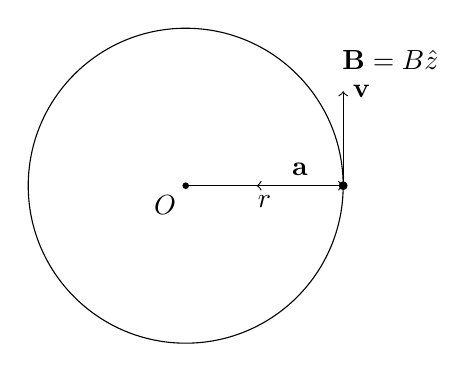
\begin{tikzpicture}[scale=1.0]
\draw (0,0) circle (2);
\fill (0,0) circle (1.2pt);
\draw (0,0) node[below left] {$O$};
\fill (2,0) circle (1.6pt);
\draw[->] (0,0) -- (2,0) node[midway, below] {$r$};
\draw[->] (2,0) -- (2,1.2) node[right] {$\mathbf v$};
\draw[->] (2,0) -- (0.9,0) node[midway, above] {$\mathbf a$};
\draw (2.6,1.6) node {$\mathbf B=B\hat z$};
\end{tikzpicture}
\caption{Uniform circular motion in the plane transverse to a uniform magnetic field. This is an editorial schematic, included to make the final geometric step explicit.}
\end{figure}

Let \(r\) be the radius of the orbit. Then
\begin{align}
|\mathbf a|=\frac{v^2}{r},
\qquad
|\mathbf v\times\mathbf B|=vB,
\end{align}
so the magnitude of the force law gives
\begin{align}
m\frac{v^2}{r}=\frac{e}{c}vB.
\end{align}
Cancel one power of \(v\), and the radius is
\begin{align}
r=\frac{mcv}{eB}.
\end{align}
The lecture briefly drops the factor of \(c\) and then restores it. With the convention \(m\mathbf a=\frac{e}{c}\mathbf v\times\mathbf B\), the expression above is the consistent one.

What the field does not determine is the center of the circle. Any point in the plane may serve as the center of an orbit, and different speeds produce different radii. The field fixes the relation between \(r\) and \(v\), not the position of the guiding center.

\section{Closing Questions and Limits of the Formalism}

The lecture ends by widening the frame rather than extending the central derivation, and that rhythm is worth preserving. Several natural questions appear here.

First, canonical momentum is not directly measurable. The directly physical momentum is the mechanical momentum \(m\mathbf v\), and its components are gauge invariant. The canonical momentum depends on the gauge, but it is the variable the Hamiltonian formalism requires. That is the price of using the powerful phase-space machinery.

Second, Maxwell's equations are not being derived in this chapter. The fields are treated as fixed backgrounds. To make the electromagnetic field dynamical one must add the field part of the action as well. Only then does one see the full interaction between particles and fields, and only then can questions about gauge symmetry and conserved quantities be asked in the complete system.

\subsection{Question \& Answer}

\paragraph{Question.} What happens if \(\nabla\!\cdot\!\mathbf B\neq 0\)?

\paragraph{Answer.} Then the simple vector-potential construction breaks down. One cannot globally write \(\mathbf B=\nabla\times\mathbf A\), and the elementary magnetic Lagrangian used here no longer follows. One may still declare
\begin{align}
m\mathbf a=\frac{e}{c}\mathbf v\times\mathbf B
\end{align}
to be the equation of motion, and classically that is a perfectly serviceable rule. But it would no longer arise from this simple action principle. For quantum mechanics that loss would be much more serious.

This is the point at which the lecture briefly returns to magnetic monopoles. The transcript garbles one sentence into ``\(\nabla\!\cdot p=0\),'', but the intended statement is clearly that one of Maxwell's equations in ordinary electrodynamics is
\begin{align}
\nabla\!\cdot\!\mathbf B=0.
\end{align}
If magnetic monopoles exist, new physics must enter. The lecture treats that topic only as a boundary marker for the present formalism, not as part of the main derivation.

Finally, there are brief historical remarks about quaternions. They are interesting, but separate. They do not belong to the central chain of reasoning that runs from the vector potential to gauge invariance, from the Lagrangian to the Lorentz force, and from the Hamiltonian to circular motion.

One late remark deserves to be retained almost verbatim in spirit. In classical mechanics one could say: never mind the action principle, just write down the Newton--Lorentz equations and move on. That is true as far as it goes. But the lecture insists, correctly, that for the deeper formal structure---and especially for quantum mechanics---there is no real way around the vector potential.

\section{Summary}

The lecture opens with the divergence-free constraint on magnetic fields and immediately turns that constraint into a construction:
\begin{align}
\nabla\!\cdot\!\mathbf B=0,
\qquad
\mathbf B=\nabla\times\mathbf A.
\end{align}
The cost is gauge ambiguity, and the response is the principle of gauge invariance. Once the magnetic particle Lagrangian
\begin{align}
L=\frac{1}{2}mv^2+\frac{e}{c}\mathbf A\cdot\mathbf v
\end{align}
is written down, the Euler--Lagrange equations slowly reorganize themselves into the Lorentz force law
\begin{align}
m\mathbf a=\frac{e}{c}\mathbf v\times\mathbf B.
\end{align}
The Hamiltonian then reveals a subtle but decisive point: as a function of \((\mathbf x,\mathbf p)\) it is modified by the magnetic field, but numerically it is still just \(\frac{1}{2}mv^2\), so the speed remains constant. Finally, by choosing gauges intelligently in the uniform-field example, we see the motion unfold in the most concrete possible way: the particle moves in a circle in the \(xy\)-plane, with radius
\begin{align}
r=\frac{mcv}{eB}.
\end{align}
The chapter as a whole follows the lecture's own rhythm: solve a constraint, accept an ambiguity, identify the invariant content, and then return to the geometry of an actual orbit.